\chapter{F-4 Pitch Attitude Control}\label{c:f4}
\section{Introduction} 

This chapter outlines a fuzzy PID system for the approach condition of an F-4 fighter jet. The F4 stands in
for more modern jets with fly-by-wire systems, and was chosen because the equations of motion were available.
The task at hand is to design a pitch attitude hold controller for the F4 that is robust
enough at be used across the entire flight envelope without modification. The controller was designed for the
approach condition due to its complexity.

The main challenge of this problem lies in the fact that the flight conditions that a
fighter jet experiences are wide and varied. It is not feasible to design and implement an optimal
controller for each one individually. A common approach to this situation would be to derive a gain schedule which
allows the controller to automatically adjust the linear gains to meet the control needs at any time. However,
the
approach explored in this chapter is to train a GFS to determine a set of PID gains based on state feedback.
This allows the controller to adapt to new flight situations similarly to a PID gain schedule, but without the
need to explicitly tune a PID controller for each case.

\section{Fuzzy PID} While seeking to design a controller robust enough to be used across the entire flight
envelope, the approach condition was chosen for its challenging dynamics. Once the controller is tuned for the
approach condition , it is tested across many off-design cases to determine its
robustness. The cases chosen for robustness analysis are the approach condition with a 50\% reduction in
aerodynamic coefficients , subsonic cruise condition , and the
supersonic cruise condition (see \cref{t:f4eoms}). Each of these scenarios presents a challenging dynamic
control problem with poles very close to the right half of the plane. Fuzzy logic is well-suited to this task
in that it will allow the control gains to move around in a way which may keep the poles in the left half of
the plane. The system dynamics studied here were used by Bossert and Cohen\cite{bossert2002pid} to design both 
a PID and a Fuzzy controller, which will be used as benchmarks. The equations for the four scenarios

{
\renewcommand*{\arraystretch}{3}
\begin{table}
    \centering
    \caption{Transfer functions for various flight conditions of the F-4 fighter jet}\label{t:f4eoms}
    \begin{tabular}{|c|c|}\hline
        \textbf{Flight Condition}                                     & \textbf{Transfer Function}\\\hline
     Approach                                                & $\displaystyle\frac{3361s^2 + 1357s + 102.2}{230.6s^5 +
     2508s^4+2161s^2 + 63.04s + 32.01}$\\\hline
     Approach 50\% deg & $\displaystyle\frac{3361 s^2 + 1372s + 105}{230.6s^5 +
     2472s^4 + 1731s^3 + 744.8s^2 + 36.92s + 16}$\\\hline
     Subsonic Cruise                                         & $\displaystyle\frac{\num{9.99e4}s^2 + \num{5.105e4}s +
     623.4}{877.6s^5 + 9884s^4 + \num{1.82e4}s^3 + \num{7.114e4}s^2 - 61.19s - 114.1}$\\\hline
     Supersonic Cruise                                       & $\displaystyle\frac{\num{1.3e5}s^2 + \num{2.183e4}s -
     31.29}{1742s^5 + \num{1.83e4}s^4 + \num{3.553e4}s^3 + \num{2.677e5}s^2 + 1247s + 123.9}$\\\hline
\end{tabular}
\end{table}
}

One large downside to fuzzy systems are that they require a significant expense of effort to tune. This task
becomes even more cumbersome with an increase of membership functions, which, in turn, increase the number of
rules (possibly exponentially). The FIS designer is then relegated to either drawing on a store of heuristic
knowledge or experience (perhaps from an expert), or to trial-and-error iteration to incrementally improve the
controller. The method used here is a GA which plays the part of automating and guiding the
trial-and-error process (see next section). This method effectively circumvents the difficulty of tuning a FIS,
and makes the job of controlling this near-unstable system more feasible.

\section{System Controller Design Methodology} At first, an attempt was made to utilize
Simulink\textsuperscript{\textregistered} and \textsc{Matlab}\textsuperscript{\textregistered} to design a
genetic algorithm (GA) which would simulate the plant transfer functions with a fuzzy-PID controller in the
feedback loop. The GA, written in \textsc{Matlab}, would call the Simulink model and evaluate the performance
of the controller. This methodology presented a number of problems to the designer. The Simulink Fuzzy Logic
Block seemed to slow down the execution of the control loop siginificantly, making a single simulation run up
to an order of magnitude slower than one with only PID control. This shortcoming can be circumvented by using
a lookup table in place of the fuzzy controller, but the overhead time needed to generate the lookup table
negates the simulation speed gains.

In light of the issues with using a Simulink GA, the GA was implemented in traditional \textsc{Matlab} using
\verb|ODE45| as the ordinary differential equation solver; however, due to the adaptive timestep of the
solver, it is prohibitively difficult to accurately obtain error derivative and integral terms for use in the
PID controller. This led the author to eventually write a simple ordinary differential equation solver in
\textsc{Matlab} which gives access to all errors at each time step, but the execution of a single simulation
was expectedly and prohibitively slow.

As a result, a genetic fuzzy system was implemented  using  the C programming language\cite{fuzzyc}.  This GA uses the
comparable rk8pd (Runge-Kutta Prince-Dormand (8,9)) stepping function from the Gnu Scientific Library (GSL) to
solve the ordinary differential equation. This method allows the user to specify some basic parameters which
are desired in the final FIS, a cost function to be applied to each solution, and some basic parameters for
the GA, at which point the GA starts generating and evaluating FIS's until a suitable stop condition has been
met.

To avoid the need to tune three individual FISs, a multi input multi output FIS was created which outputs the
three gains $K_p$, $K_i$, and $K_d$. The FIS accepts as its inputs the absolute error in elevator angle, the
error integral, and the error derivative, $e$, $e_i$, and $e_d$ respectively. To determine the quality of a
controller, a number of metrics with respect to its response to a step input are gathered as a means for
comparison. These metrics are the settling time, $T_s$, rise time, $T_r$, time to peak value, $T_p$, maximum
value, $M_p$ and final value, $FV$.

The cost function used to describe the desired controller behavior plays an integral role in the success or
failure of any evolutionary strategy. The problem of designing this fuzzy PID controller presents a nice case
study in which to observe undesired side effects of an overly simplistic cost function. The first cost function
which is implemented is simply to minimize the settling time of the system. This has the side effect of
increasing the overshoot of the elevator pitch angle. The cost function is then adjusted to take into account
the overshoot and yields a more amenable response behavior.

\section{Results for Nominal and Other Flight Conditions}

\Cref{f:f4} shows the responses of the aircraft to the fuzzy PID controller as
trained by a GA using the simple minimal settling time cost function. This cost function yields a significant
overshoot as an outcome. To lessen the magnitude of this effect, the GA was given a new cost function which
places a higher premium on overshoot, yielding a more amenable result, as shown in \cref{f:f4_nos}.

\begin{figure}[ht]
    \centering
    \begin{subfigmatrix}{2}
        \subfigure[\label{f:f4_nominal}Nominal approach condition]
            {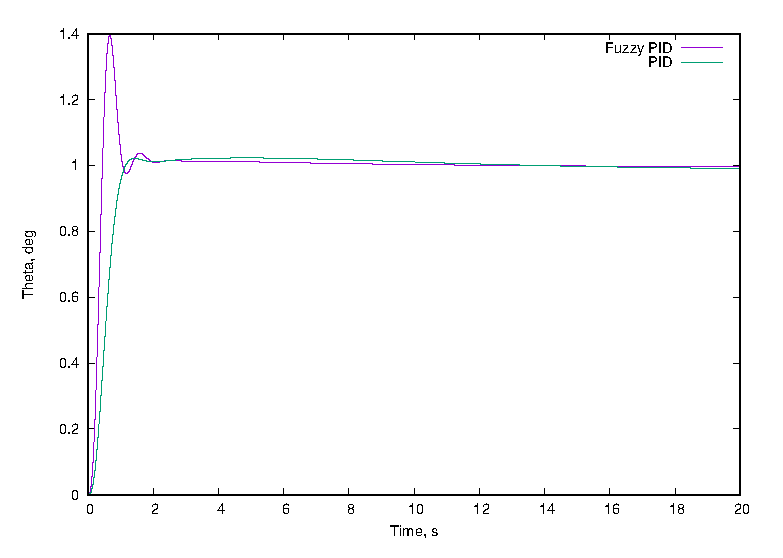
\includegraphics[width=0.49\textwidth]{results/f4_approach}}
        \subfigure[\label{f:f4_degraded}Degraded aerodynamic derivative approach condition]
            {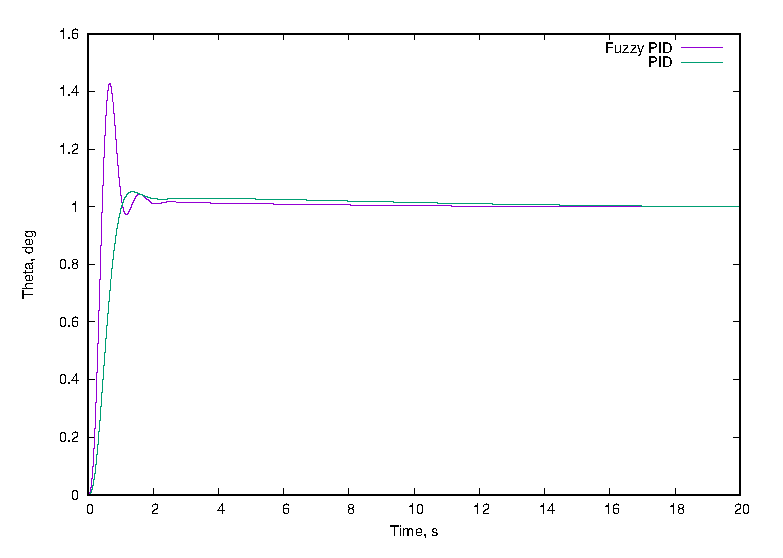
\includegraphics[width=0.49\textwidth]{results/f4_deg}}
        \subfigure[\label{f:f4_subsonic}Subsonic cruise condition]
            {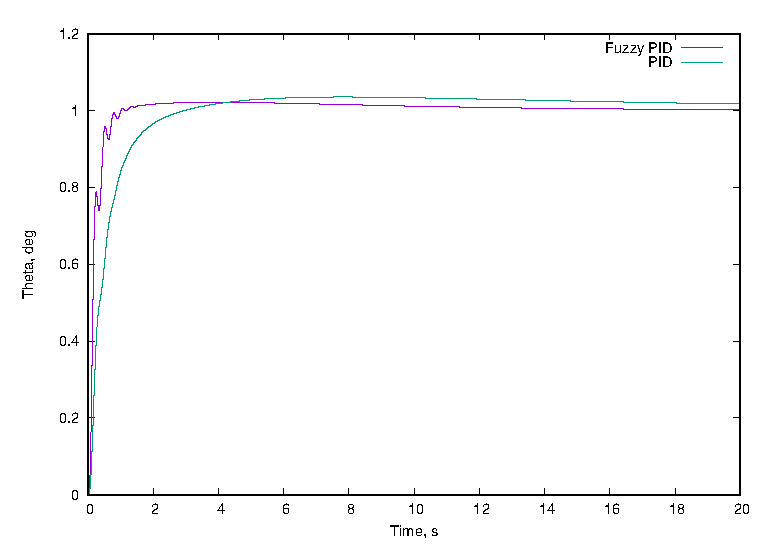
\includegraphics[width=0.49\textwidth]{results/f4_sub}}
        \subfigure[\label{f:f4_supersonic}Supersonic cruise condition]
            {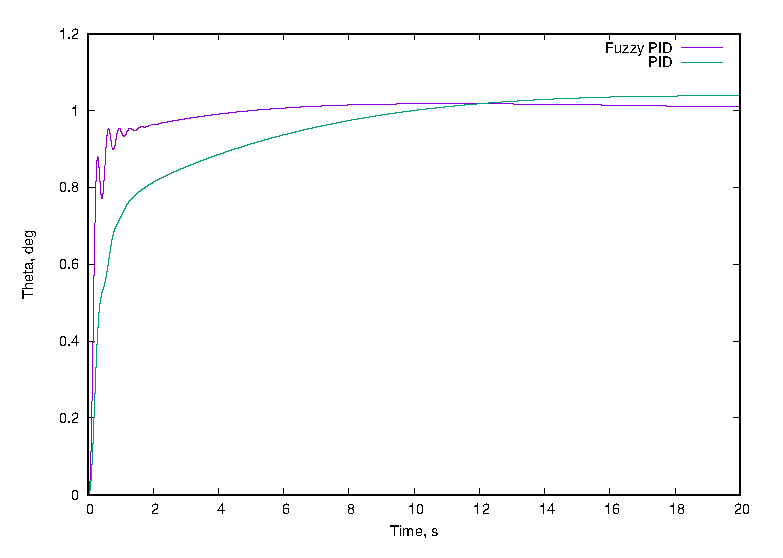
\includegraphics[width=0.49\textwidth]{results/f4_sup}}
    \end{subfigmatrix} \caption{Step response for various flight conditions. Note the increased overshoot for
                                nominal conditions from the Fuzzy-PID controller.}\label{f:f4}
\end{figure}

\begin{figure}[ht]
    \centering 
    \begin{subfigmatrix}{2}
        \subfigure[\label{f:f4_nominal_nos}Nominal approach condition]
            {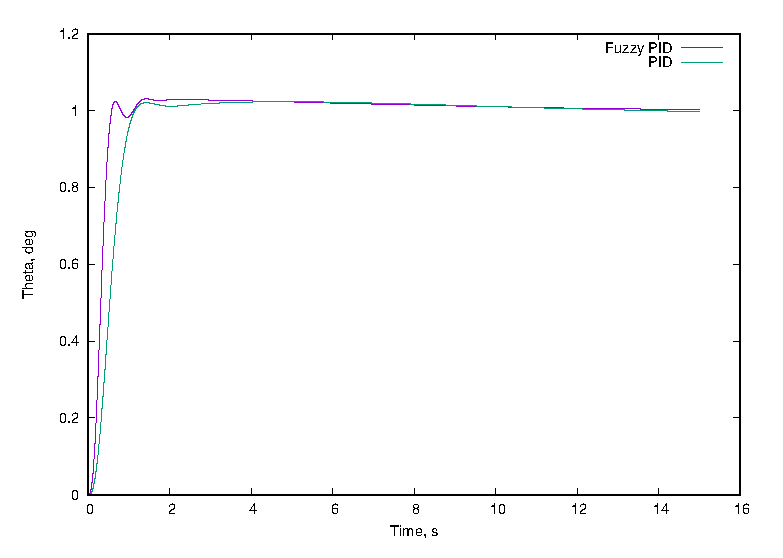
\includegraphics[width=0.49\textwidth]{results/test/f4_approach}}
        \subfigure[\label{f:f4_degraded_nos}Degraded aerodynamic derivative approach condition]
            {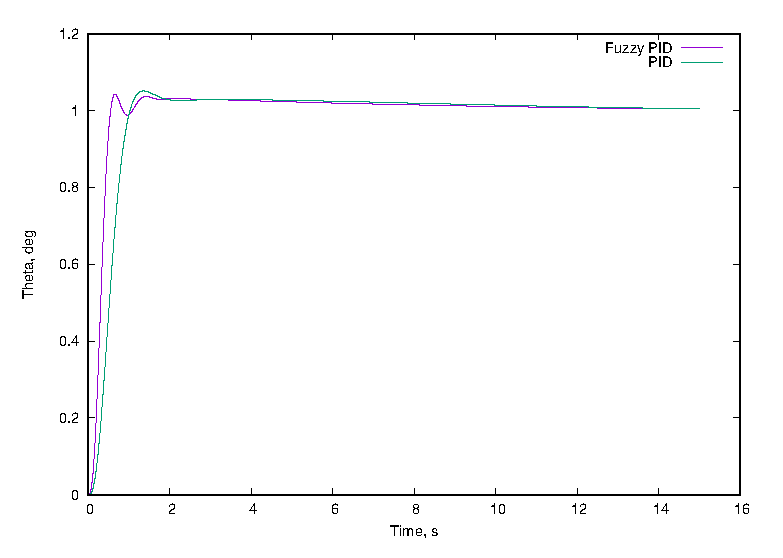
\includegraphics[width=0.49\textwidth]{results/test/f4_deg}}
        \subfigure[\label{f:f4_subsonic_nos}Subsonic cruise condition]
            {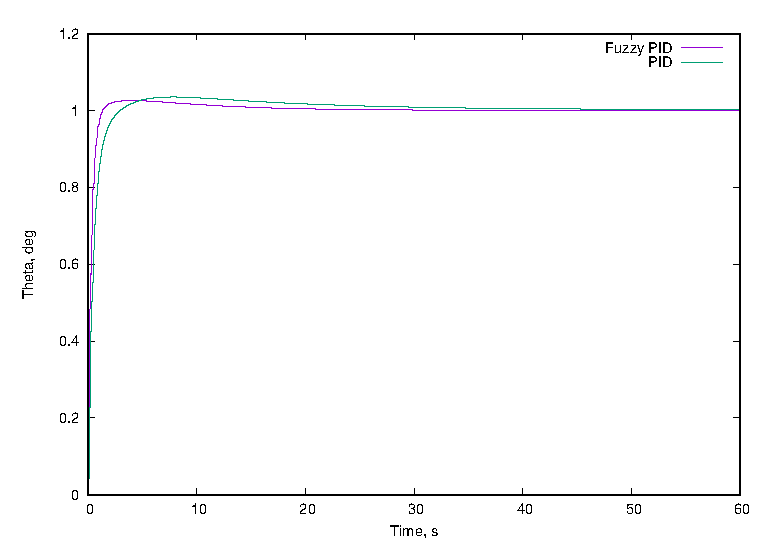
\includegraphics[width=0.49\textwidth]{results/test/f4_sub}}
        \subfigure[\label{f:f4_supersonic_nos}Supersonic cruise condition]
            {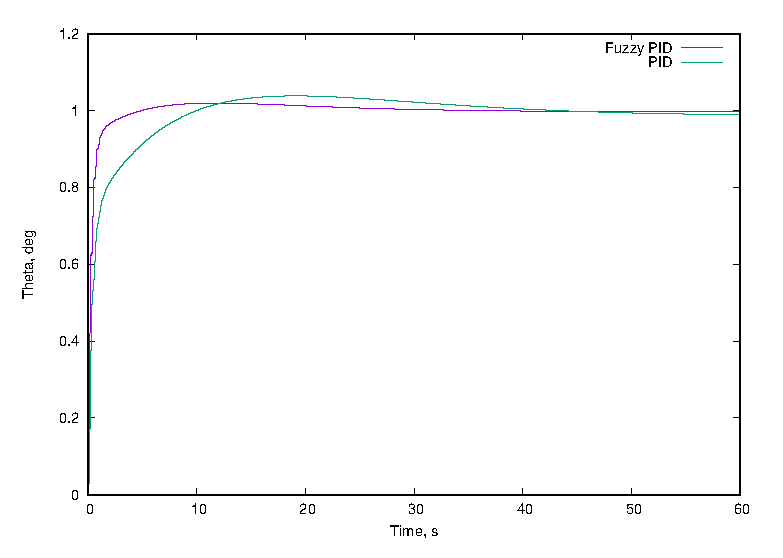
\includegraphics[width=0.49\textwidth]{results/test/f4_sup}}
    \end{subfigmatrix}
    \caption{Step response for various flight conditions using the controller created with modified cost
        function. Note the significantly decreased overshoot for nominal and degraded flight
    conditions.}\label{f:f4_nos}
\end{figure}

\begin{sidewaystable}
    \centering
    \caption{Comparison table of current results with those of Bossert and Cohen}\label{t:f4}
    \begin{tabular}{|c|c|c|c|c|c|}\hline
        Case
            & $T_s$ (s) & $T_r$ (s) & $T_p$ (s) & $M_p$ (deg) & FV (deg) \\\hline
        Root Locus F4 Approach (Design Condition)
            & 23.6      & 1.09      & 3.14      & 1.09        & 0.62 \\\hline
        PID F4 Approach (Design Condition)
            & 7.08      & 1.27      & 4.98      & 1.023       & 1.00 \\\hline
        Fuzzy F4 Approach (Design Condition)
            & 1.65      & 1.68      & 1.74      & 1.013       & 1.00 \\\hline
        \textbf{Fuzzy PID Approach (Design Condition)}
            & 1.86 & 0.26 & 0.66 & 1.396 & 1.00\\\hline

        Root Locus 50\% Red in $C_{m\alpha}$ and $C_{mq}$
            & 25.8      & 1.16      & 3.57      & 1.42        & 0.77 \\\hline
        PID 50\% Red in $C_{m\alpha}$ and $C_{mq}$
            & 8.0       & 1.03      & 1.35      & 1.045       & 1.01 \\\hline
        Fuzzy 50\% Red in $C_{m\alpha}$ and $C_{mq}$
            & 1.66      & 1.69      & 1.75      & 1.014       & 1.00 \\\hline
        \textbf{Fuzzy PID 50\% Red in $C_{m\alpha}$ and $C_{mq}$}
            & 1.87 & 0.25 & 0.66 & 1.428 & 1.00\\\hline

    \end{tabular}
    \bigskip
    \bigskip
    \bigskip
    \caption{Resulting FIS response from GA with modified cost function}\label{t:f4_nos}
    \begin{tabular}{|c|c|c|c|c|c|}\hline
        Case & $T_s$ (s) & $T_r$ (s) & $T_p$ (s) & $M_p$ (deg) & FV (deg) \\\hline
        Fuzzy PID Approach (Design Condition) & 4.96 & 0.34 & 1.43 & 1.031 & 1.00\\\hline

        Fuzzy PID 50\% Red in $C_{m\alpha}$ and $C_{mq}$ & 4.47 & 0.33 & 0.66 & 1.043 & 1.00\\\hline

    \end{tabular}
\end{sidewaystable}

\begin{table}[ht]
    \centering
    \caption{Comparison of response times for subsonic and supersonic cruise conditions for original and
             modified cost function. Modifying the cost function showed no improvements for this set of
             conditions, rather only proved to slow the response time with no gain in overshoot.}%
             \label{t:subsup}
    \begin{tabular}{|c|c|c|c|c|c|}\hline
        Case & $T_s$ (s) & $T_r$ (s) & $T_p$ (s) &
        $M_p$ (deg) & FV (deg) \\\hline Subsonic Cruise (Orig. Cost) & 0.93 & 0.38 & 3.91 & 1.022 & 1.00\\\hline
 Supersonic Cruise (Orig.
        Cost) & 3.84 & 0.73 & 11.10 & 1.018 & 1.01\\\hline
 Subsonic Cruise (Mod. Cost) & 7.97 & 0.59 & 4.09 & 1.026 & 1.00\\\hline
 Supersonic Cruise (Mod.
        Cost) & 15.53 & 0.73 & 11.74 & 1.020 & 1.00\\\hline

    \end{tabular}
\end{table}


As can be seen from \crefrange{t:f4}{t:f4_nos}, the settling time of the step response is significantly
slower when training a controller using the new cost function. However, the overall response is arguably better due
to the reduced overshoot. Additionally, though not nearly as good for the nominal and degraded flight conditions as was Bossert and
Cohen's solution, the response for the subsonic and supersonic cruise conditions show arguably better
performance (see \cref{t:subsup}).

\section{Conclusion}
In order to demonstrate the flexibility of a fuzzy PID controller, a controller was designed to meet the
demands of the approach condition of an F4 fighter. It was shown that this controller exhibited good behavior
across a wider domain than that in which it was trained. This demonstrates that an adaptive fuzzy PID
controller can be an effective approach to problems with a wide variety of scenarios.

Future will work include assessing the response of the aircraft to fuzzy PID control according to the C*
criterion, Gibson's drop back criterion, and other flying qualities standards\cite{standard1990flying}. This will provide a richer
assessment of the controller's performance.
